\documentclass[]{article}
\usepackage{lmodern}
\usepackage{amssymb,amsmath}
\usepackage{ifxetex,ifluatex}
\usepackage{fixltx2e} % provides \textsubscript
\ifnum 0\ifxetex 1\fi\ifluatex 1\fi=0 % if pdftex
  \usepackage[T1]{fontenc}
  \usepackage[utf8]{inputenc}
\else % if luatex or xelatex
  \ifxetex
    \usepackage{mathspec}
  \else
    \usepackage{fontspec}
  \fi
  \defaultfontfeatures{Ligatures=TeX,Scale=MatchLowercase}
\fi
% use upquote if available, for straight quotes in verbatim environments
\IfFileExists{upquote.sty}{\usepackage{upquote}}{}
% use microtype if available
\IfFileExists{microtype.sty}{%
\usepackage{microtype}
\UseMicrotypeSet[protrusion]{basicmath} % disable protrusion for tt fonts
}{}
\usepackage[margin=1in]{geometry}
\usepackage{hyperref}
\hypersetup{unicode=true,
            pdftitle={SI},
            pdfborder={0 0 0},
            breaklinks=true}
\urlstyle{same}  % don't use monospace font for urls
\usepackage{graphicx,grffile}
\makeatletter
\def\maxwidth{\ifdim\Gin@nat@width>\linewidth\linewidth\else\Gin@nat@width\fi}
\def\maxheight{\ifdim\Gin@nat@height>\textheight\textheight\else\Gin@nat@height\fi}
\makeatother
% Scale images if necessary, so that they will not overflow the page
% margins by default, and it is still possible to overwrite the defaults
% using explicit options in \includegraphics[width, height, ...]{}
\setkeys{Gin}{width=\maxwidth,height=\maxheight,keepaspectratio}
\IfFileExists{parskip.sty}{%
\usepackage{parskip}
}{% else
\setlength{\parindent}{0pt}
\setlength{\parskip}{6pt plus 2pt minus 1pt}
}
\setlength{\emergencystretch}{3em}  % prevent overfull lines
\providecommand{\tightlist}{%
  \setlength{\itemsep}{0pt}\setlength{\parskip}{0pt}}
\setcounter{secnumdepth}{0}
% Redefines (sub)paragraphs to behave more like sections
\ifx\paragraph\undefined\else
\let\oldparagraph\paragraph
\renewcommand{\paragraph}[1]{\oldparagraph{#1}\mbox{}}
\fi
\ifx\subparagraph\undefined\else
\let\oldsubparagraph\subparagraph
\renewcommand{\subparagraph}[1]{\oldsubparagraph{#1}\mbox{}}
\fi

%%% Use protect on footnotes to avoid problems with footnotes in titles
\let\rmarkdownfootnote\footnote%
\def\footnote{\protect\rmarkdownfootnote}

%%% Change title format to be more compact
\usepackage{titling}

% Create subtitle command for use in maketitle
\providecommand{\subtitle}[1]{
  \posttitle{
    \begin{center}\large#1\end{center}
    }
}

\setlength{\droptitle}{-2em}

  \title{SI}
    \pretitle{\vspace{\droptitle}\centering\huge}
  \posttitle{\par}
    \author{}
    \preauthor{}\postauthor{}
      \predate{\centering\large\emph}
  \postdate{\par}
    \date{14 August 2019}

\usepackage{booktabs}
\usepackage{longtable}
\usepackage{array}
\usepackage{multirow}
\usepackage{wrapfig}
\usepackage{float}
\usepackage{colortbl}
\usepackage{pdflscape}
\usepackage{tabu}
\usepackage{threeparttable}
\usepackage{threeparttablex}
\usepackage[normalem]{ulem}
\usepackage{makecell}
\usepackage{xcolor}

\begin{document}
\maketitle

{
\setcounter{tocdepth}{2}
\tableofcontents
}
\hypertarget{additional-control-variable-choices}{%
\section{Additional control variable
choices}\label{additional-control-variable-choices}}

For additional robustness checks, we considered the following
indicators:

\begin{itemize}
\tightlist
\item
  Media freedom, from Whitten-Woodring and Van Belle, 2015, ``The
  Correlates of Media Freedom'', \emph{PSRM}, via
  \url{http://faculty.uml.edu/Jenifer_whittenwoodring/MediaFreedomData_000.aspx}.
  Per the authors recommendations we collapsed the 3-valued media
  freedom indicator into a binary ``functionally free'' and ``not free''
  version.
\item
  IGO membership as an indicator of political globalization, from the
  COW IGO state unit dataset.
\item
  Linear and squared year trends
\item
  Human rights organization membership (\texttt{hro\_n}) and secretariat
  locations (\texttt{hro\_secloc}). From Murdie and Davis 2012 ``Shaming
  and Blaming'', ISQ, \url{http://amandamurdie.org/research.html}, where
  the original variable names are \texttt{hrfilled} and
  \texttt{HRsecretariatlocation}.
\item
  Trade as \% of GDP as an economic globalization indicator. From the
  World Bank WDI.
\end{itemize}

The trade and HRO data contain missing values. The number of
observations in a model depend on the particular combination of the 3
indicators impacted in a given specification, such that:

\begin{table}[H]
\centering
\begin{tabular}{lrr}
\toprule
Variables & N & Fraction\\
\midrule
None & 1654 & 100\\
NE.TRD.GNFS.ZS & 1552 & 94\\
hro\_n & 1209 & 73\\
hro\_secloc & 1208 & 73\\
hro\_n, NE.TRD.GNFS.ZS & 1136 & 69\\
\addlinespace
hro\_n, hro\_secloc & 971 & 59\\
hro\_n, hro\_secloc, NE.TRD.GNFS.ZS & 947 & 57\\
\bottomrule
\end{tabular}
\end{table}

Since any coefficient estimate differences between a model that includes
one or more of these three variables with missing values and another
without, we decided to not use them. Thus we restrict our sensitivity
analysis to the first three items in the list above.

\hypertarget{sensitivity-analysis}{%
\section{Sensitivity analysis}\label{sensitivity-analysis}}

The conduct the robustness / sensitivity analysis, we followed the
``reasonable specification'' approach outlined in Simonsohn, Simmons,
and Nelson (2015). This is a method that fits in the space between
estimating a limited number of additional models for robustness checks
and extreme bounds analysis where we estimate all possible combinations
of specifications given a set of variables. Instead, they suggest
listing a set of reasonable modeling and specification choices, where
each choice is a decision between two or more alternatives, and then
estimating all combinations of those choices. In the languge of Gelman's
garden of forking paths (2013), we try to follow all paths a reasonable
modeller might take.

In spirit this is a restricted version of extreme bounds analysis, that
seeks to eliminate unreasonable specifications. For example it makes no
sense to estimate a model including both raw and logged GDP, rather we
would only want to examine one at a time.

We included the following choices in our sensitivity analysis:

\begin{itemize}
\tightlist
\item
  Model type: 2 alternatives; either a regular Poisson count model (GLM)
  or a Poisson count model with random country intercepts (GLMER).
\item
  Base terms: 2 alternatives; intercept(s) only or the basic controls,
  as discussed in the main paper.
\item
  Media freedom: 2 alternatives; no control or the global media freedom
  index
\item
  Political globalization: 3 alternatives; no control or a count of HRO
  membership or a count of HRO secretariats located in a country
\item
  Year trend: 3 alternatives; no trend, linear trend, or squared trend
\end{itemize}

Altogether this represents 72 possible specifications. The one we report
in the paper is a Poisson model with random country intercepts, includes
the base control set, but does not include any other control variables.
We examined each of the 72 specifications for each of the 14 variables
of interest using each of the 3 dependent variables.

Altogether this comes out to 3,024 estimated models. Simonsohn et al use
specification plots as the first step in interpreting the findings.
Since we still have 42 specification plots overall, we skip this and
first summarize even further by tallying, for each VOI, the number of
coefficient estimates that are negative and stastistically significant
(\(p < 0.05\)), negative but \(p > 0.05\), positive but \(p > 0.05\) and
lastly positive and significant. This is shown below in Table
\ref{tab:sens}, and next we will highlight findings regarding the main
results we present in the paper. After that will be a section where we
show what specification plots are, followed by a list of all 42.

\begin{table}[t]

\caption{\label{tab:sens}Summary of sensitivity analysis estimates}
\centering
\begin{tabular}{llrrrr}
\toprule
Variable & Outcome & neg & leanneg & leanpos & pos\\
\midrule
Democracy, 0/1 & Criminal & 66 & 0 & 3 & 3\\
Democracy, 0/1 & Dissident & 72 & 0 & 0 & 0\\
Democracy, 0/1 & Marginalized & 51 & 0 & 1 & 20\\
CCP Due process & Criminal & 6 & 18 & 12 & 36\\
CCP Due process & Dissident & 39 & 15 & 0 & 18\\
\addlinespace
CCP Due process & Marginalized & 45 & 5 & 4 & 18\\
CCP Habeas corpus & Criminal & 0 & 7 & 18 & 47\\
CCP Habeas corpus & Dissident & 72 & 0 & 0 & 0\\
CCP Habeas corpus & Marginalized & 36 & 5 & 26 & 5\\
CCP Pretrial release & Criminal & 36 & 0 & 0 & 36\\
\addlinespace
CCP Pretrial release & Dissident & 63 & 0 & 0 & 9\\
CCP Pretrial release & Marginalized & 36 & 9 & 3 & 24\\
CCP Speedy trial & Criminal & 36 & 0 & 0 & 36\\
CCP Speedy trial & Dissident & 64 & 6 & 2 & 0\\
CCP Speedy trial & Marginalized & 29 & 25 & 0 & 18\\
\addlinespace
CCP Torture & Criminal & 30 & 13 & 14 & 15\\
CCP Torture & Dissident & 66 & 6 & 0 & 0\\
CCP Torture & Marginalized & 45 & 12 & 13 & 2\\
EPR Excluded groups (\% of total pop) & Criminal & 0 & 0 & 0 & 72\\
EPR Excluded groups (\% of total pop) & Dissident & 0 & 0 & 0 & 72\\
\addlinespace
EPR Excluded groups (\% of total pop) & Marginalized & 0 & 17 & 19 & 36\\
EPR Excluded groups (count) & Criminal & 0 & 7 & 9 & 56\\
EPR Excluded groups (count) & Dissident & 0 & 0 & 0 & 72\\
EPR Excluded groups (count) & Marginalized & 0 & 0 & 0 & 72\\
VDem Civil liberty social class equality & Criminal & 72 & 0 & 0 & 0\\
\addlinespace
VDem Civil liberty social class equality & Dissident & 72 & 0 & 0 & 0\\
VDem Civil liberty social class equality & Marginalized & 72 & 0 & 0 & 0\\
VDem Civil liberty social group equality & Criminal & 60 & 12 & 0 & 0\\
VDem Civil liberty social group equality & Dissident & 72 & 0 & 0 & 0\\
VDem Civil liberty social group equality & Marginalized & 72 & 0 & 0 & 0\\
\addlinespace
VDem Judicial constraints on executive & Criminal & 51 & 21 & 0 & 0\\
VDem Judicial constraints on executive & Dissident & 72 & 0 & 0 & 0\\
VDem Judicial constraints on executive & Marginalized & 69 & 0 & 0 & 3\\
VDem Legislative constraints on executive & Criminal & 30 & 4 & 32 & 6\\
VDem Legislative constraints on executive & Dissident & 72 & 0 & 0 & 0\\
\addlinespace
VDem Legislative constraints on executive & Marginalized & 36 & 22 & 11 & 3\\
VDem Power by social group & Criminal & 41 & 30 & 1 & 0\\
VDem Power by social group & Dissident & 72 & 0 & 0 & 0\\
VDem Power by social group & Marginalized & 69 & 0 & 0 & 3\\
VDem Power by socioeconomic position & Criminal & 61 & 11 & 0 & 0\\
\addlinespace
VDem Power by socioeconomic position & Dissident & 72 & 0 & 0 & 0\\
VDem Power by socioeconomic position & Marginalized & 70 & 2 & 0 & 0\\
\bottomrule
\end{tabular}
\end{table}

\hypertarget{summary-of-findings}{%
\subsection{Summary of findings}\label{summary-of-findings}}

\begin{itemize}
\tightlist
\item
  \textbf{Negative relationship for ``Democracy 0/1''}. We report a
  negative relationship between this and all three outcomes. This
  largely holds up, with significant negative estimates in all 72 specs
  for ``dissidents'', 66 for ``criminal'', and 51 for ``marginalized''
\item
  \textbf{Negative relationship for constitutional provisions}, with
  only one negative but insignificant estimate for ``CCP Habeas Corpus''
  on ``Criminal''.
\end{itemize}

\clearpage

\hypertarget{specification-plots}{%
\section{Specification plots}\label{specification-plots}}

The specification plots provide more details than our summary above
does, and also make it possible to identify, to some extent, which
specification choices lead to certain findings. Thus we include them
here for anyone interested in more detail.

\hypertarget{introduction}{%
\subsection{Introduction}\label{introduction}}

This is an example of a specification plot for the indicator of whether
a country constitution includes a due process provision
(\texttt{ccp\_dueproc}) and where the DV is ITT allegations of criminal
torture (\texttt{itt\_alleg\_vtcriminal}).

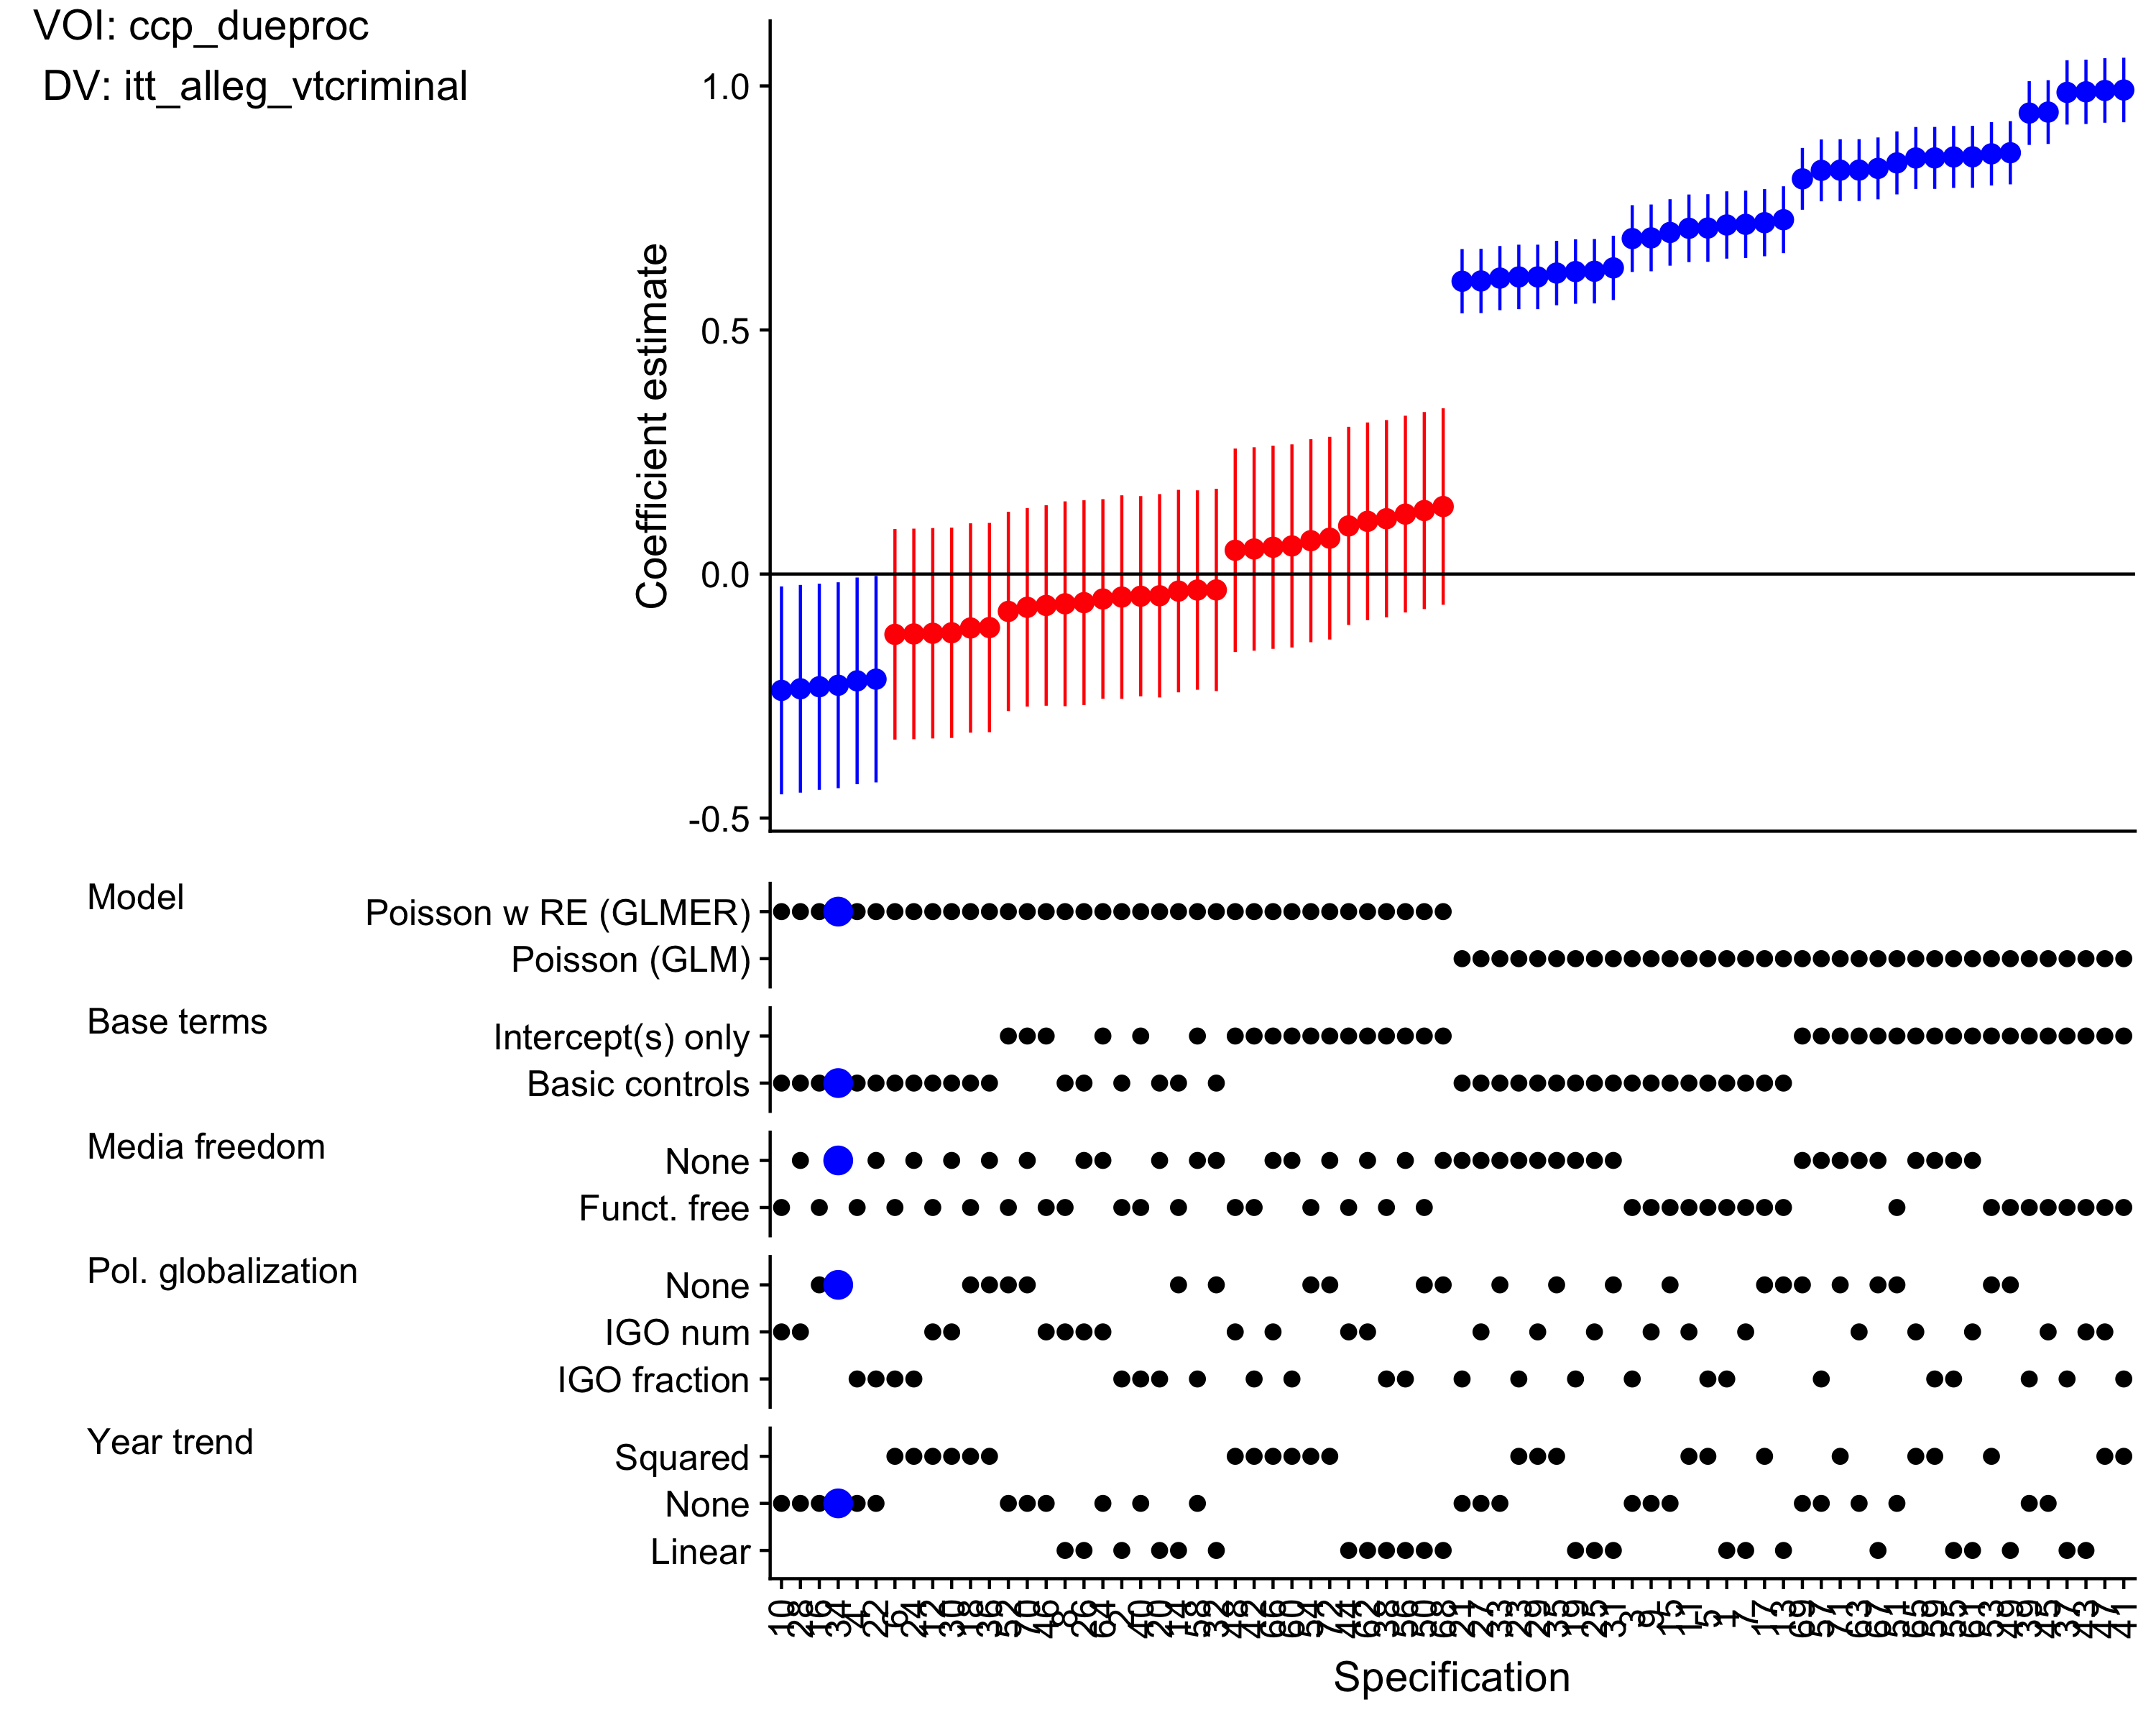
\includegraphics{../output/figures-robustness/specplot-ccp_dueproc-itt_alleg_vtcriminal.png}

The plot consists of two main elements. The panel on the top shows the
coefficient estimates for the variable of interest over a number of
different specification on the x-axis. The points and lines show point
estimates and 95\% confidence intervals; they are colored red and blue
for stastitically significant (\(p\)-value \(< 0.05\)) negative and
positive effects and grey for statisticall insignificant estimates.

The second panel at the bottom shows details for each specification. All
the way on the left are the labels for each specification choice; the
elements from which one could choose are in the next column. For example
for ``Model'' we made a choice between a regular Poisson count model
with global intercept only, versus a GLMER Poisson model that also
includes country random effects (RE). The \(x\)-axis are still
specifications, and the dots in the plot mark what choices were made in
each specification.

The specification we used in the main paper are highlighted in both
blots with the grey rectangles. We've also annotated each plot with text
in the top left that summarizes the number of significant positive or
negative, as well as insignificant, estimates.

In terms of interpretation, we can firstly see that a large but not
overwhelming proportion of estimates are positive and significant. The
patterns of dots in the specification bottom plot can give some hints at
what is driven estimate patterns. Long sequences like that for ``Model''
indicate that a specification choice is strongly related to estimates,
and indeed the positive and significant estimates are entirely due to
using a model with only a global, not country random, intercepts.
Uniform spacing on the other hand indicates that a choice plays only a
small row. This is for example the case with Media freedom when using a
Poisson RE model--the estimates change only slightly as the media
freedom indicator changes.

\hypertarget{list-of-all-specification-plots-by-voi}{%
\subsection{List of all specification plots, by
VOI}\label{list-of-all-specification-plots-by-voi}}

\hypertarget{voi-ccp_dueproc}{%
\subsection{VOI: ccp\_dueproc}\label{voi-ccp_dueproc}}

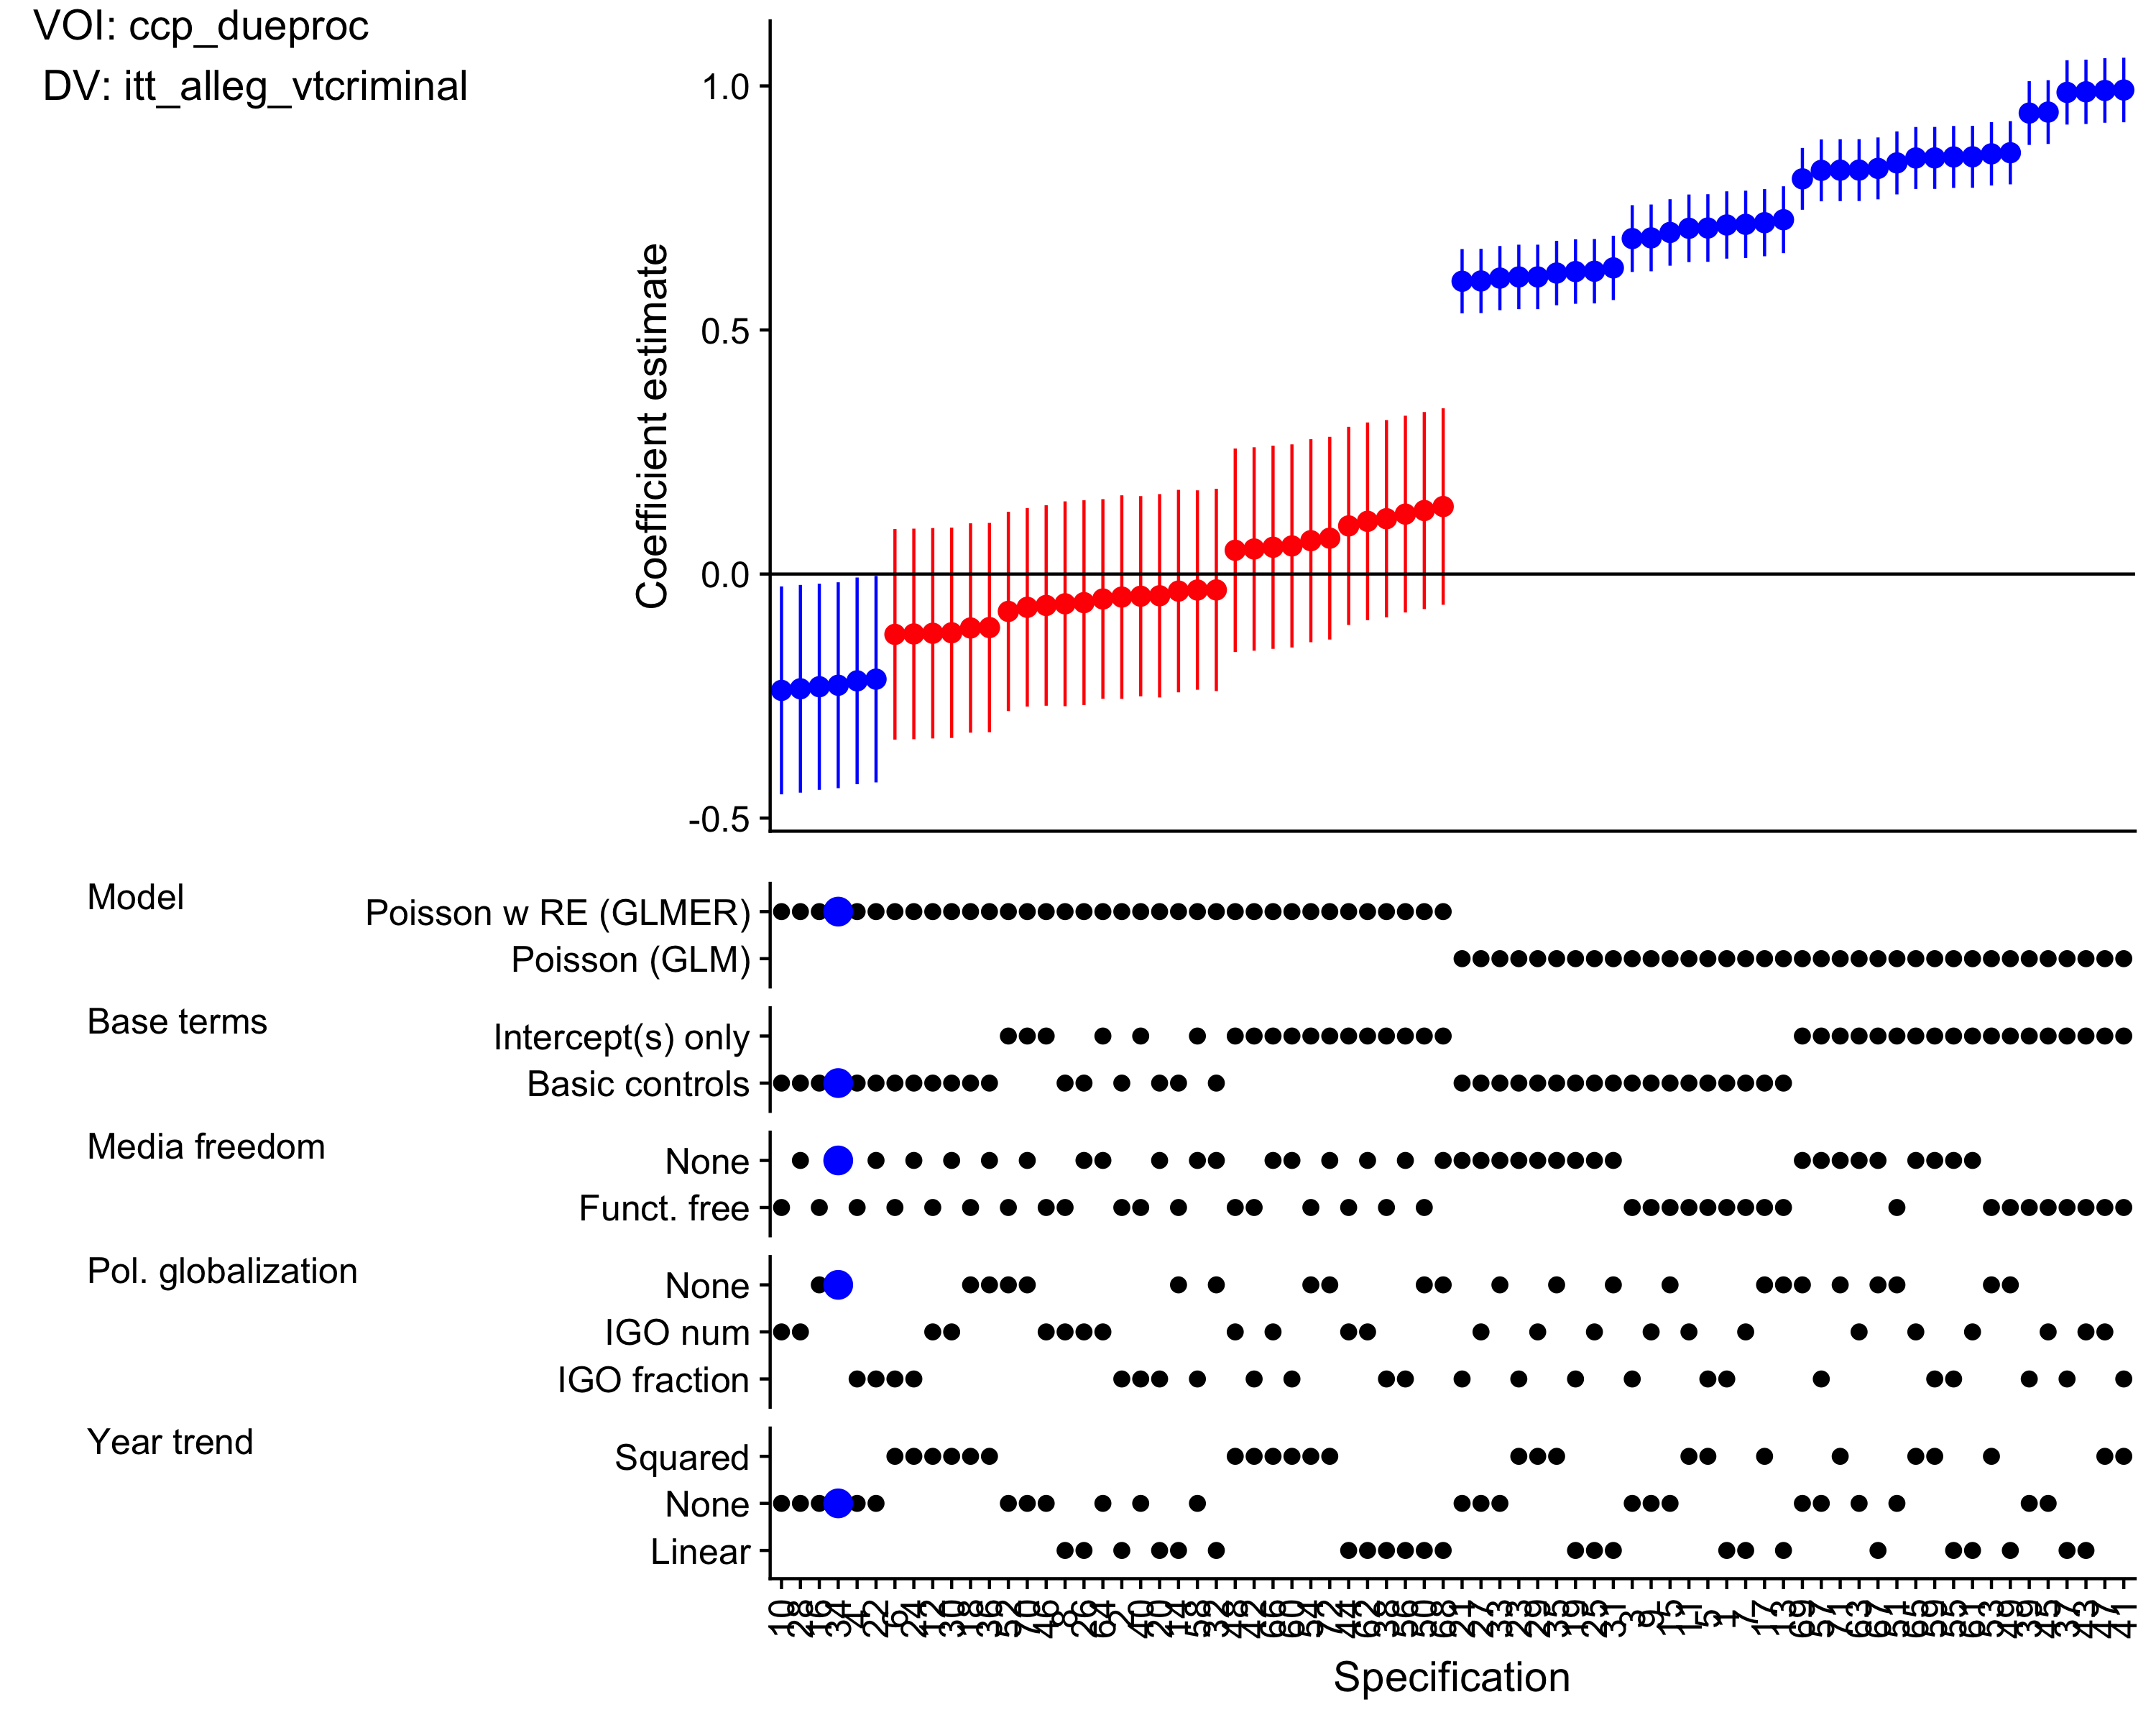
\includegraphics[height=4in]{../output/figures-robustness/specplot-ccp_dueproc-itt_alleg_vtcriminal.png}

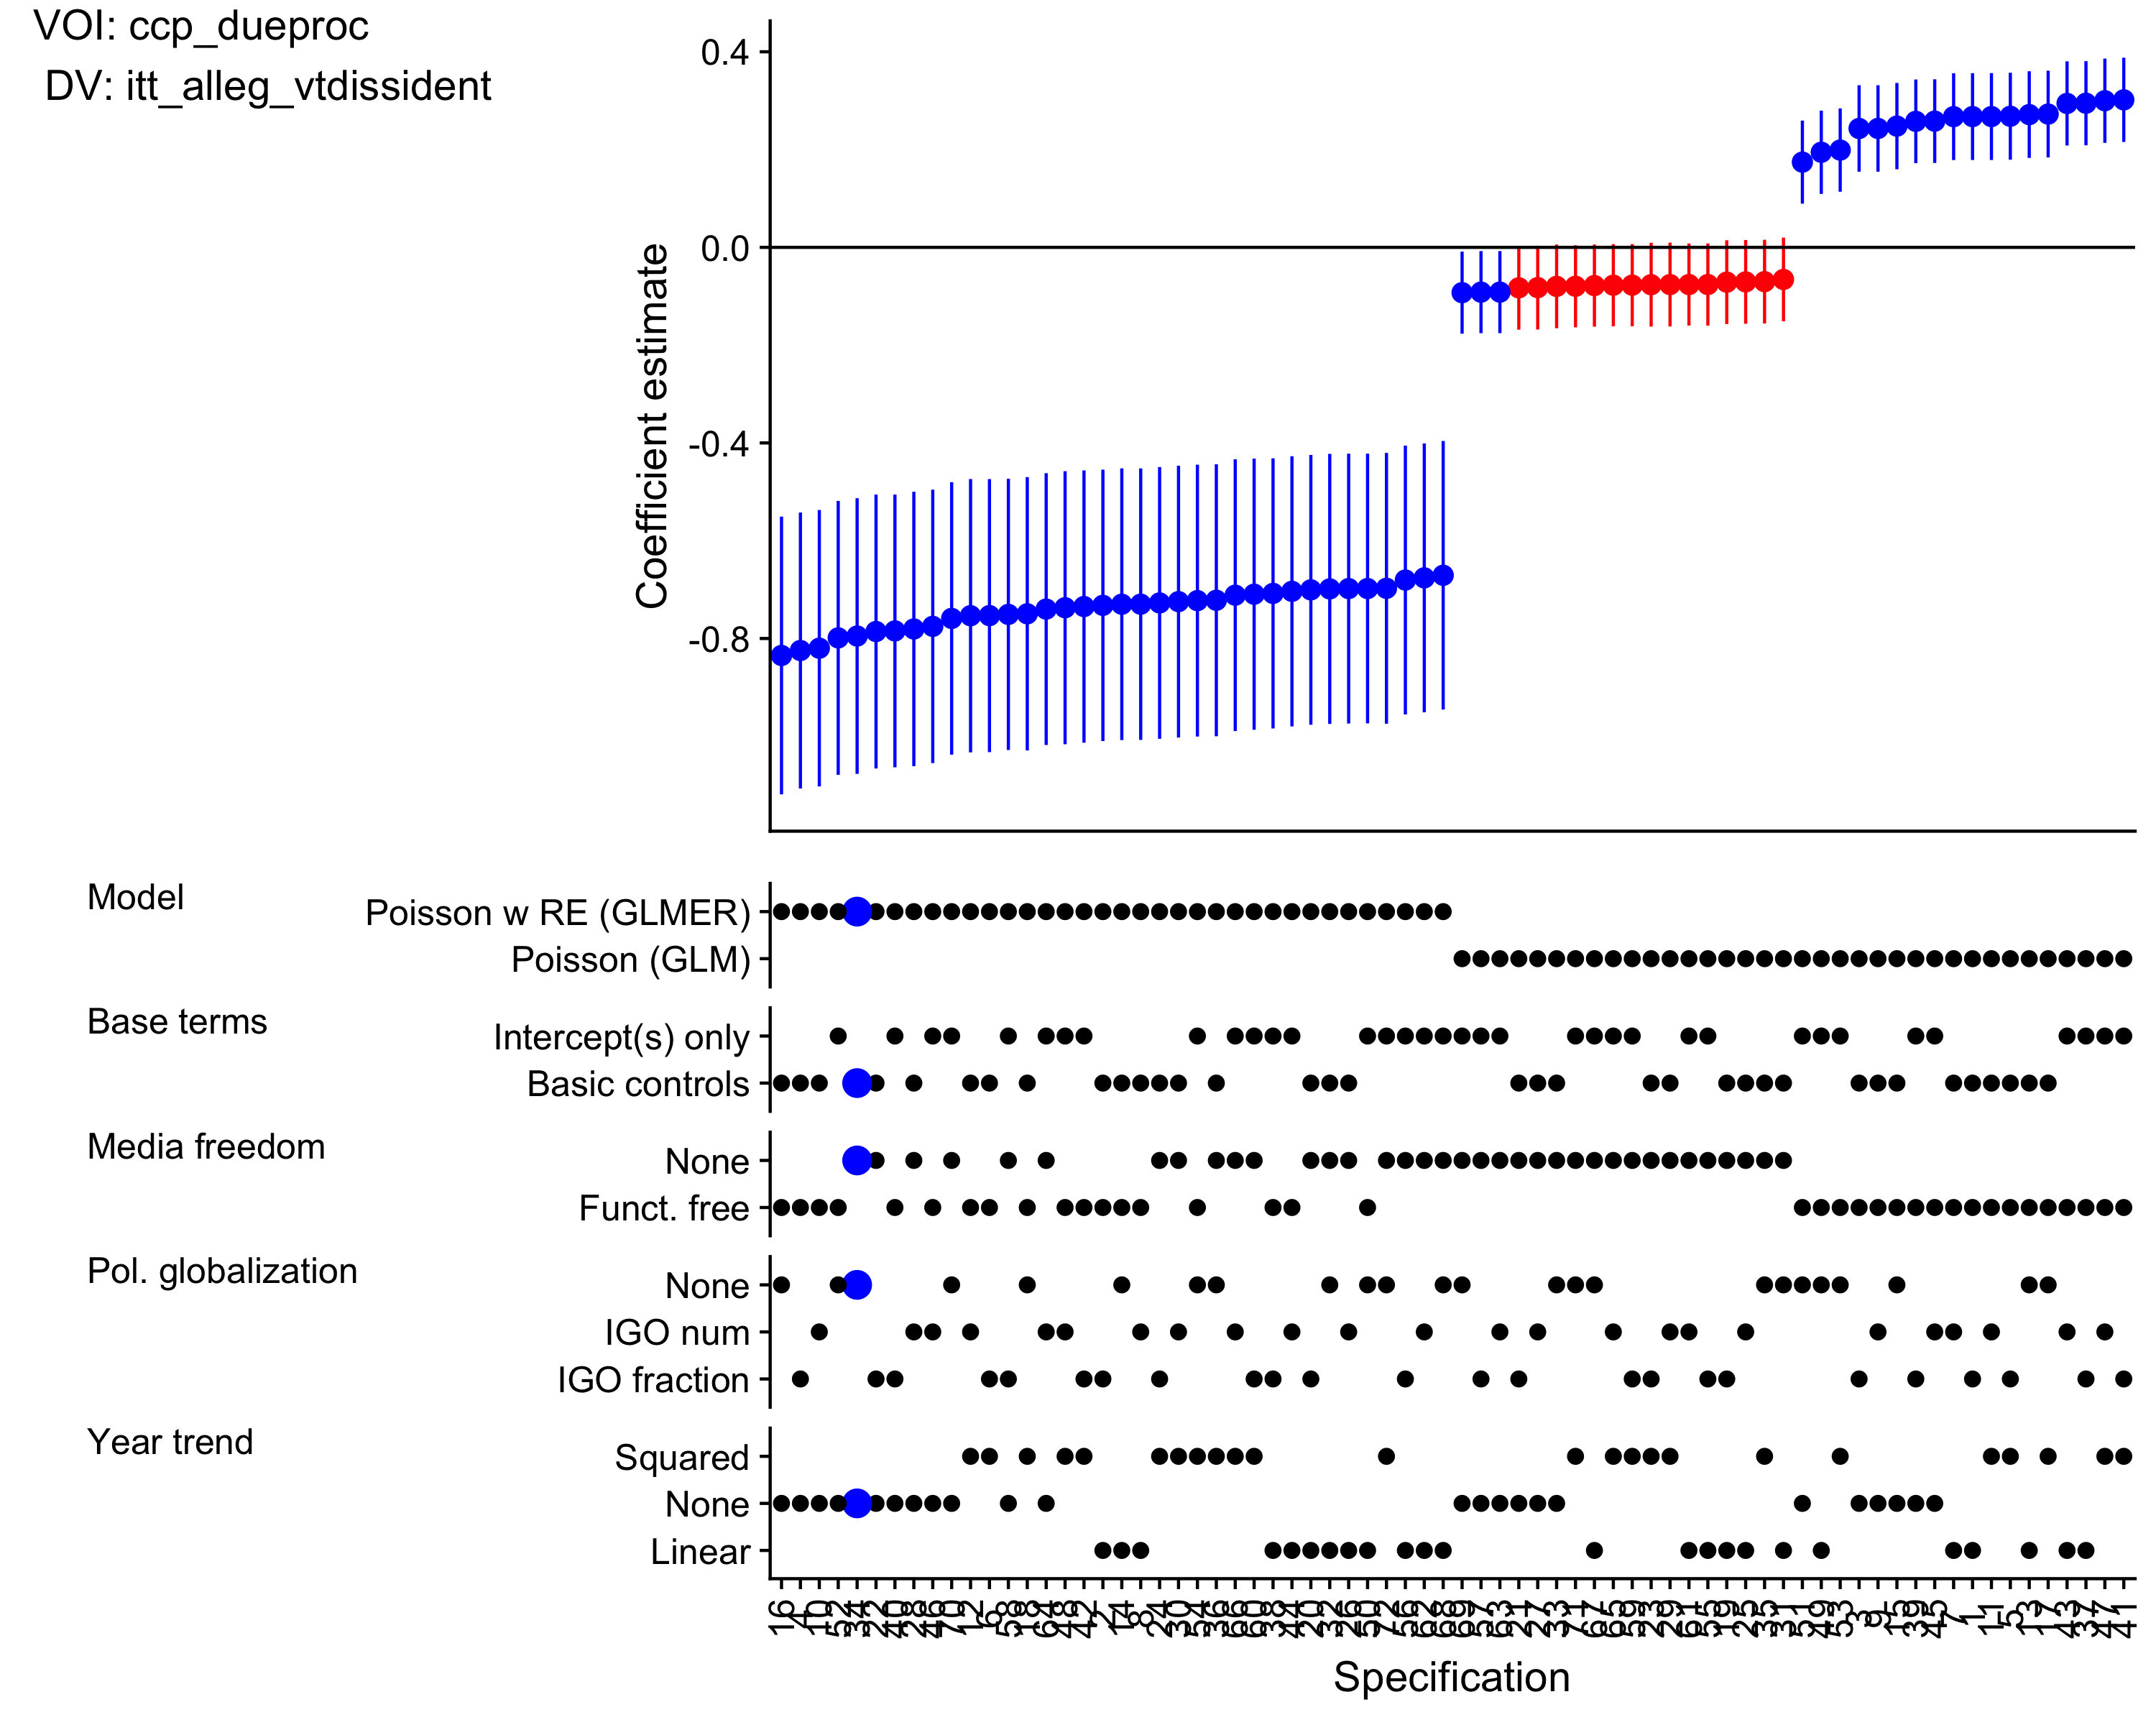
\includegraphics[height=4in]{../output/figures-robustness/specplot-ccp_dueproc-itt_alleg_vtdissident.png}

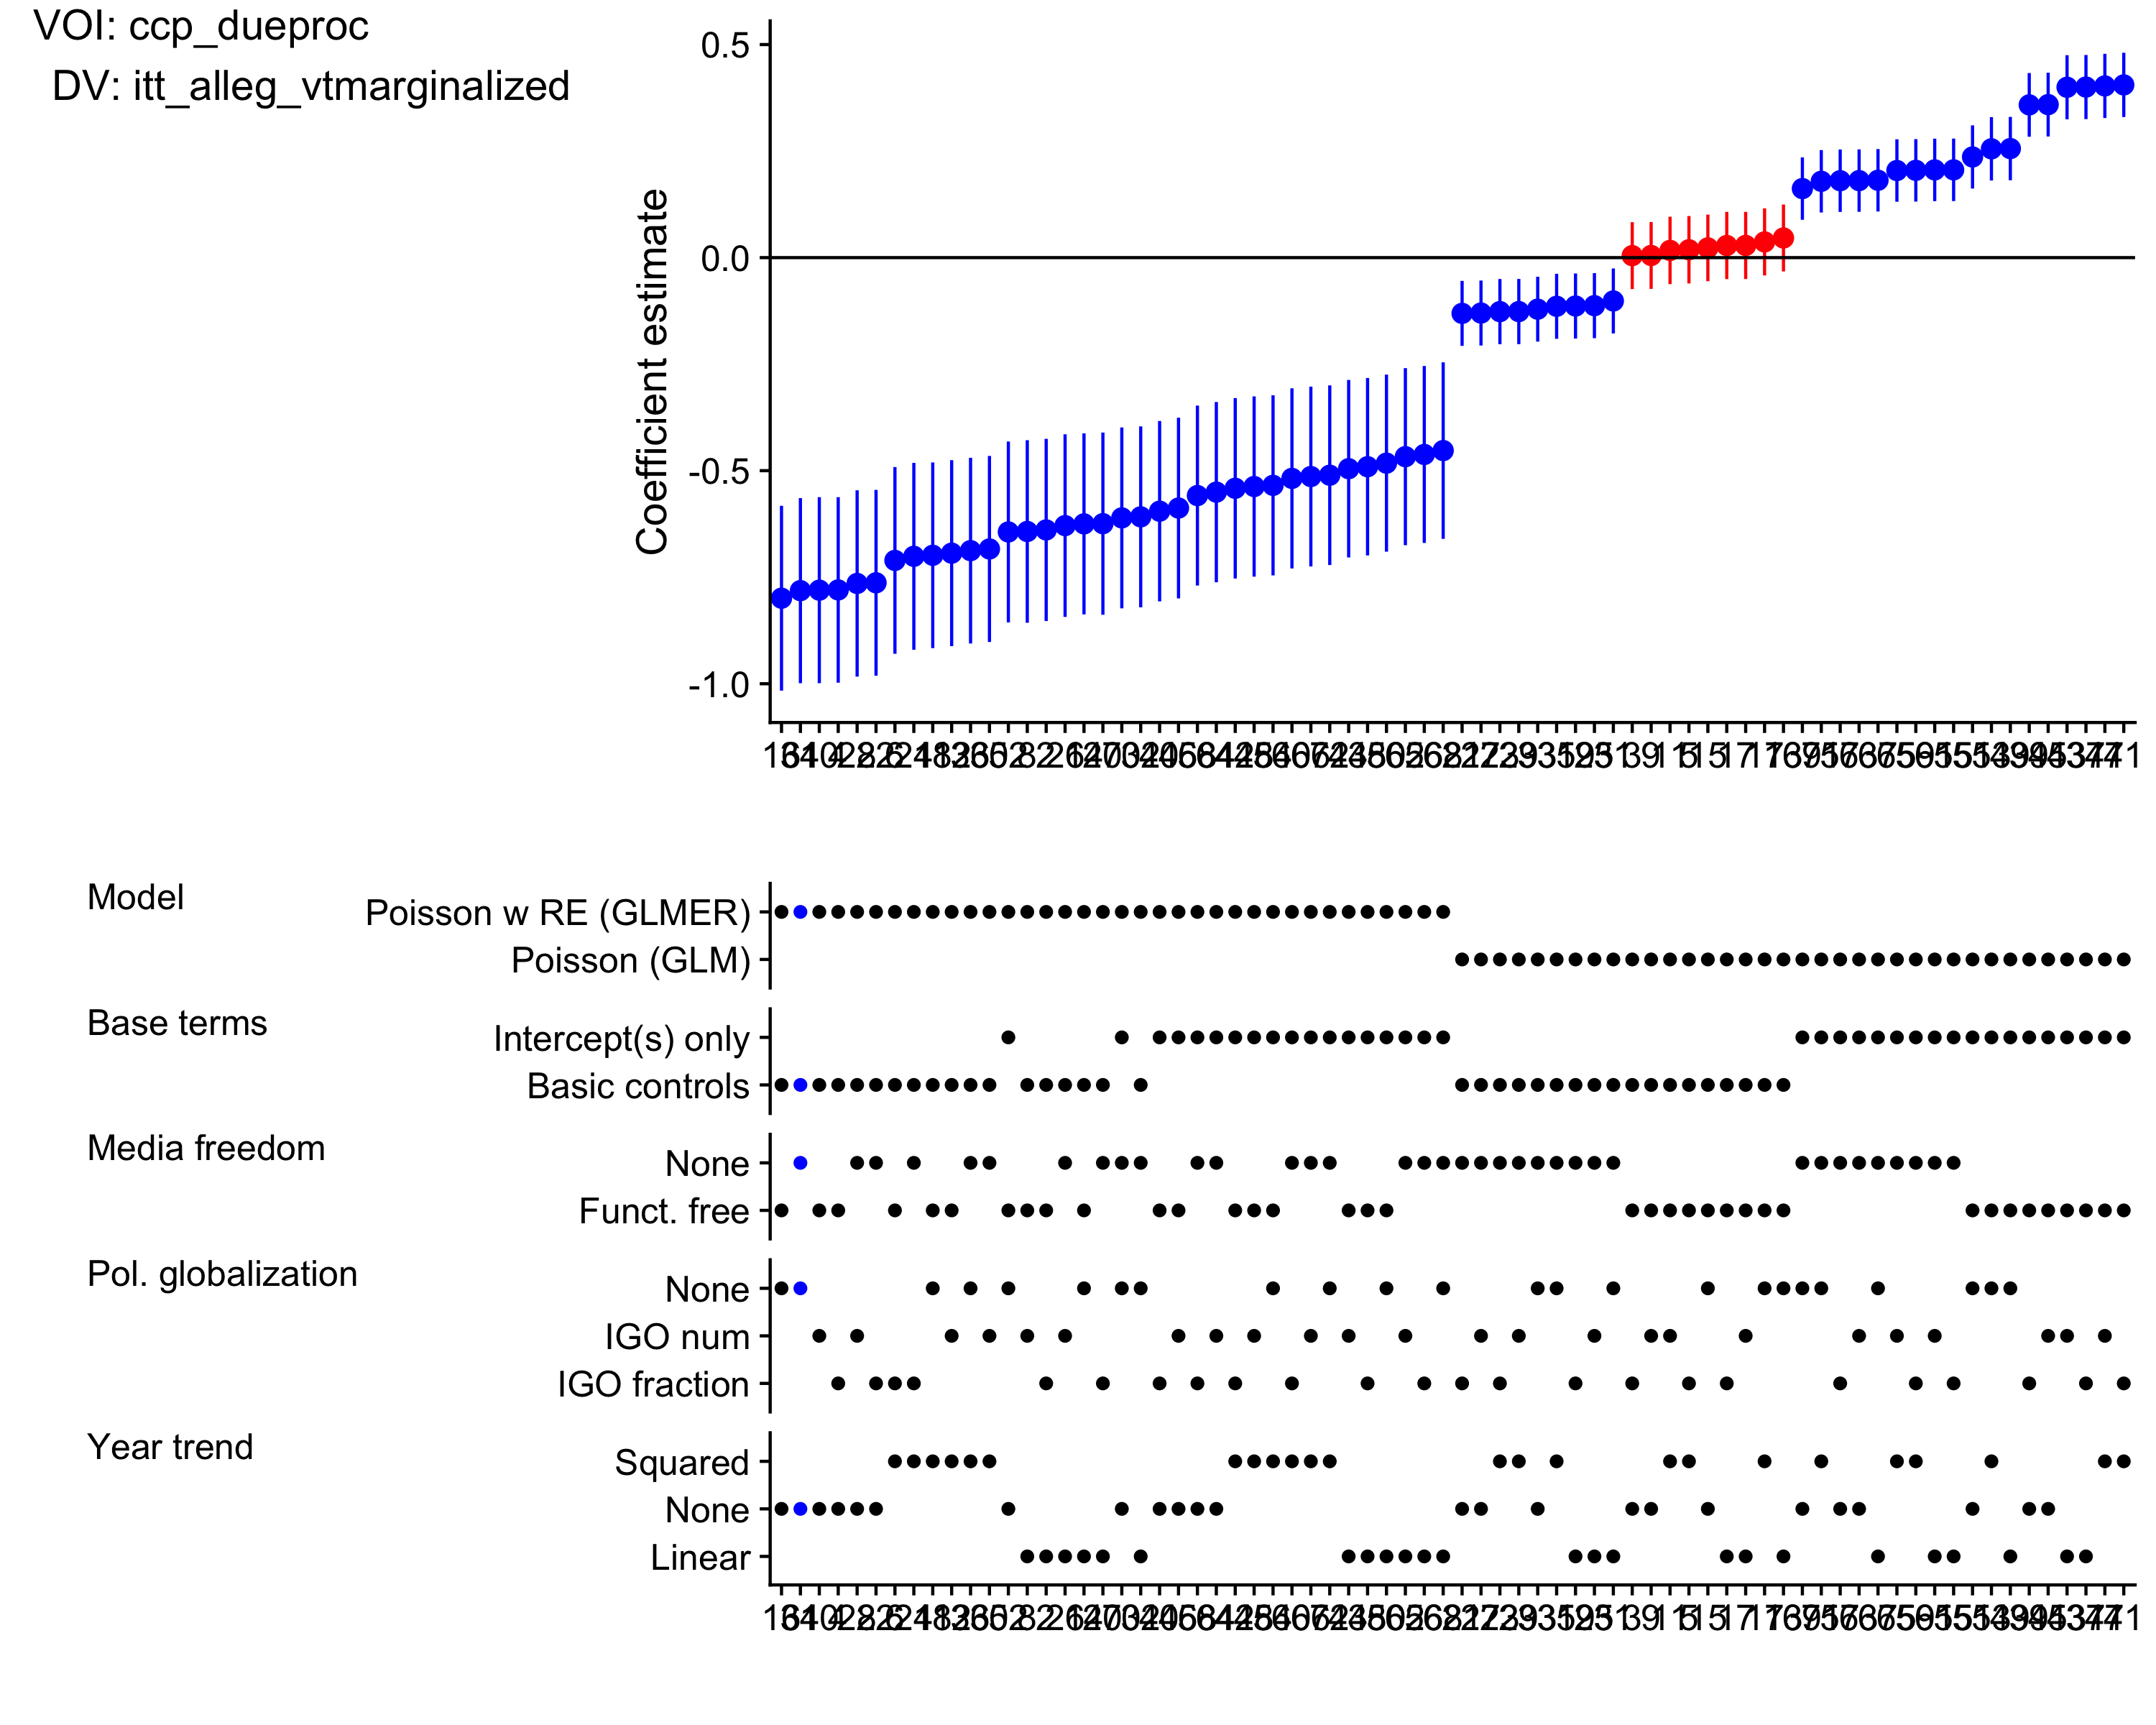
\includegraphics[height=4in]{../output/figures-robustness/specplot-ccp_dueproc-itt_alleg_vtmarginalized.png}

\hypertarget{voi-ccp_habcorp}{%
\subsection{VOI: ccp\_habcorp}\label{voi-ccp_habcorp}}

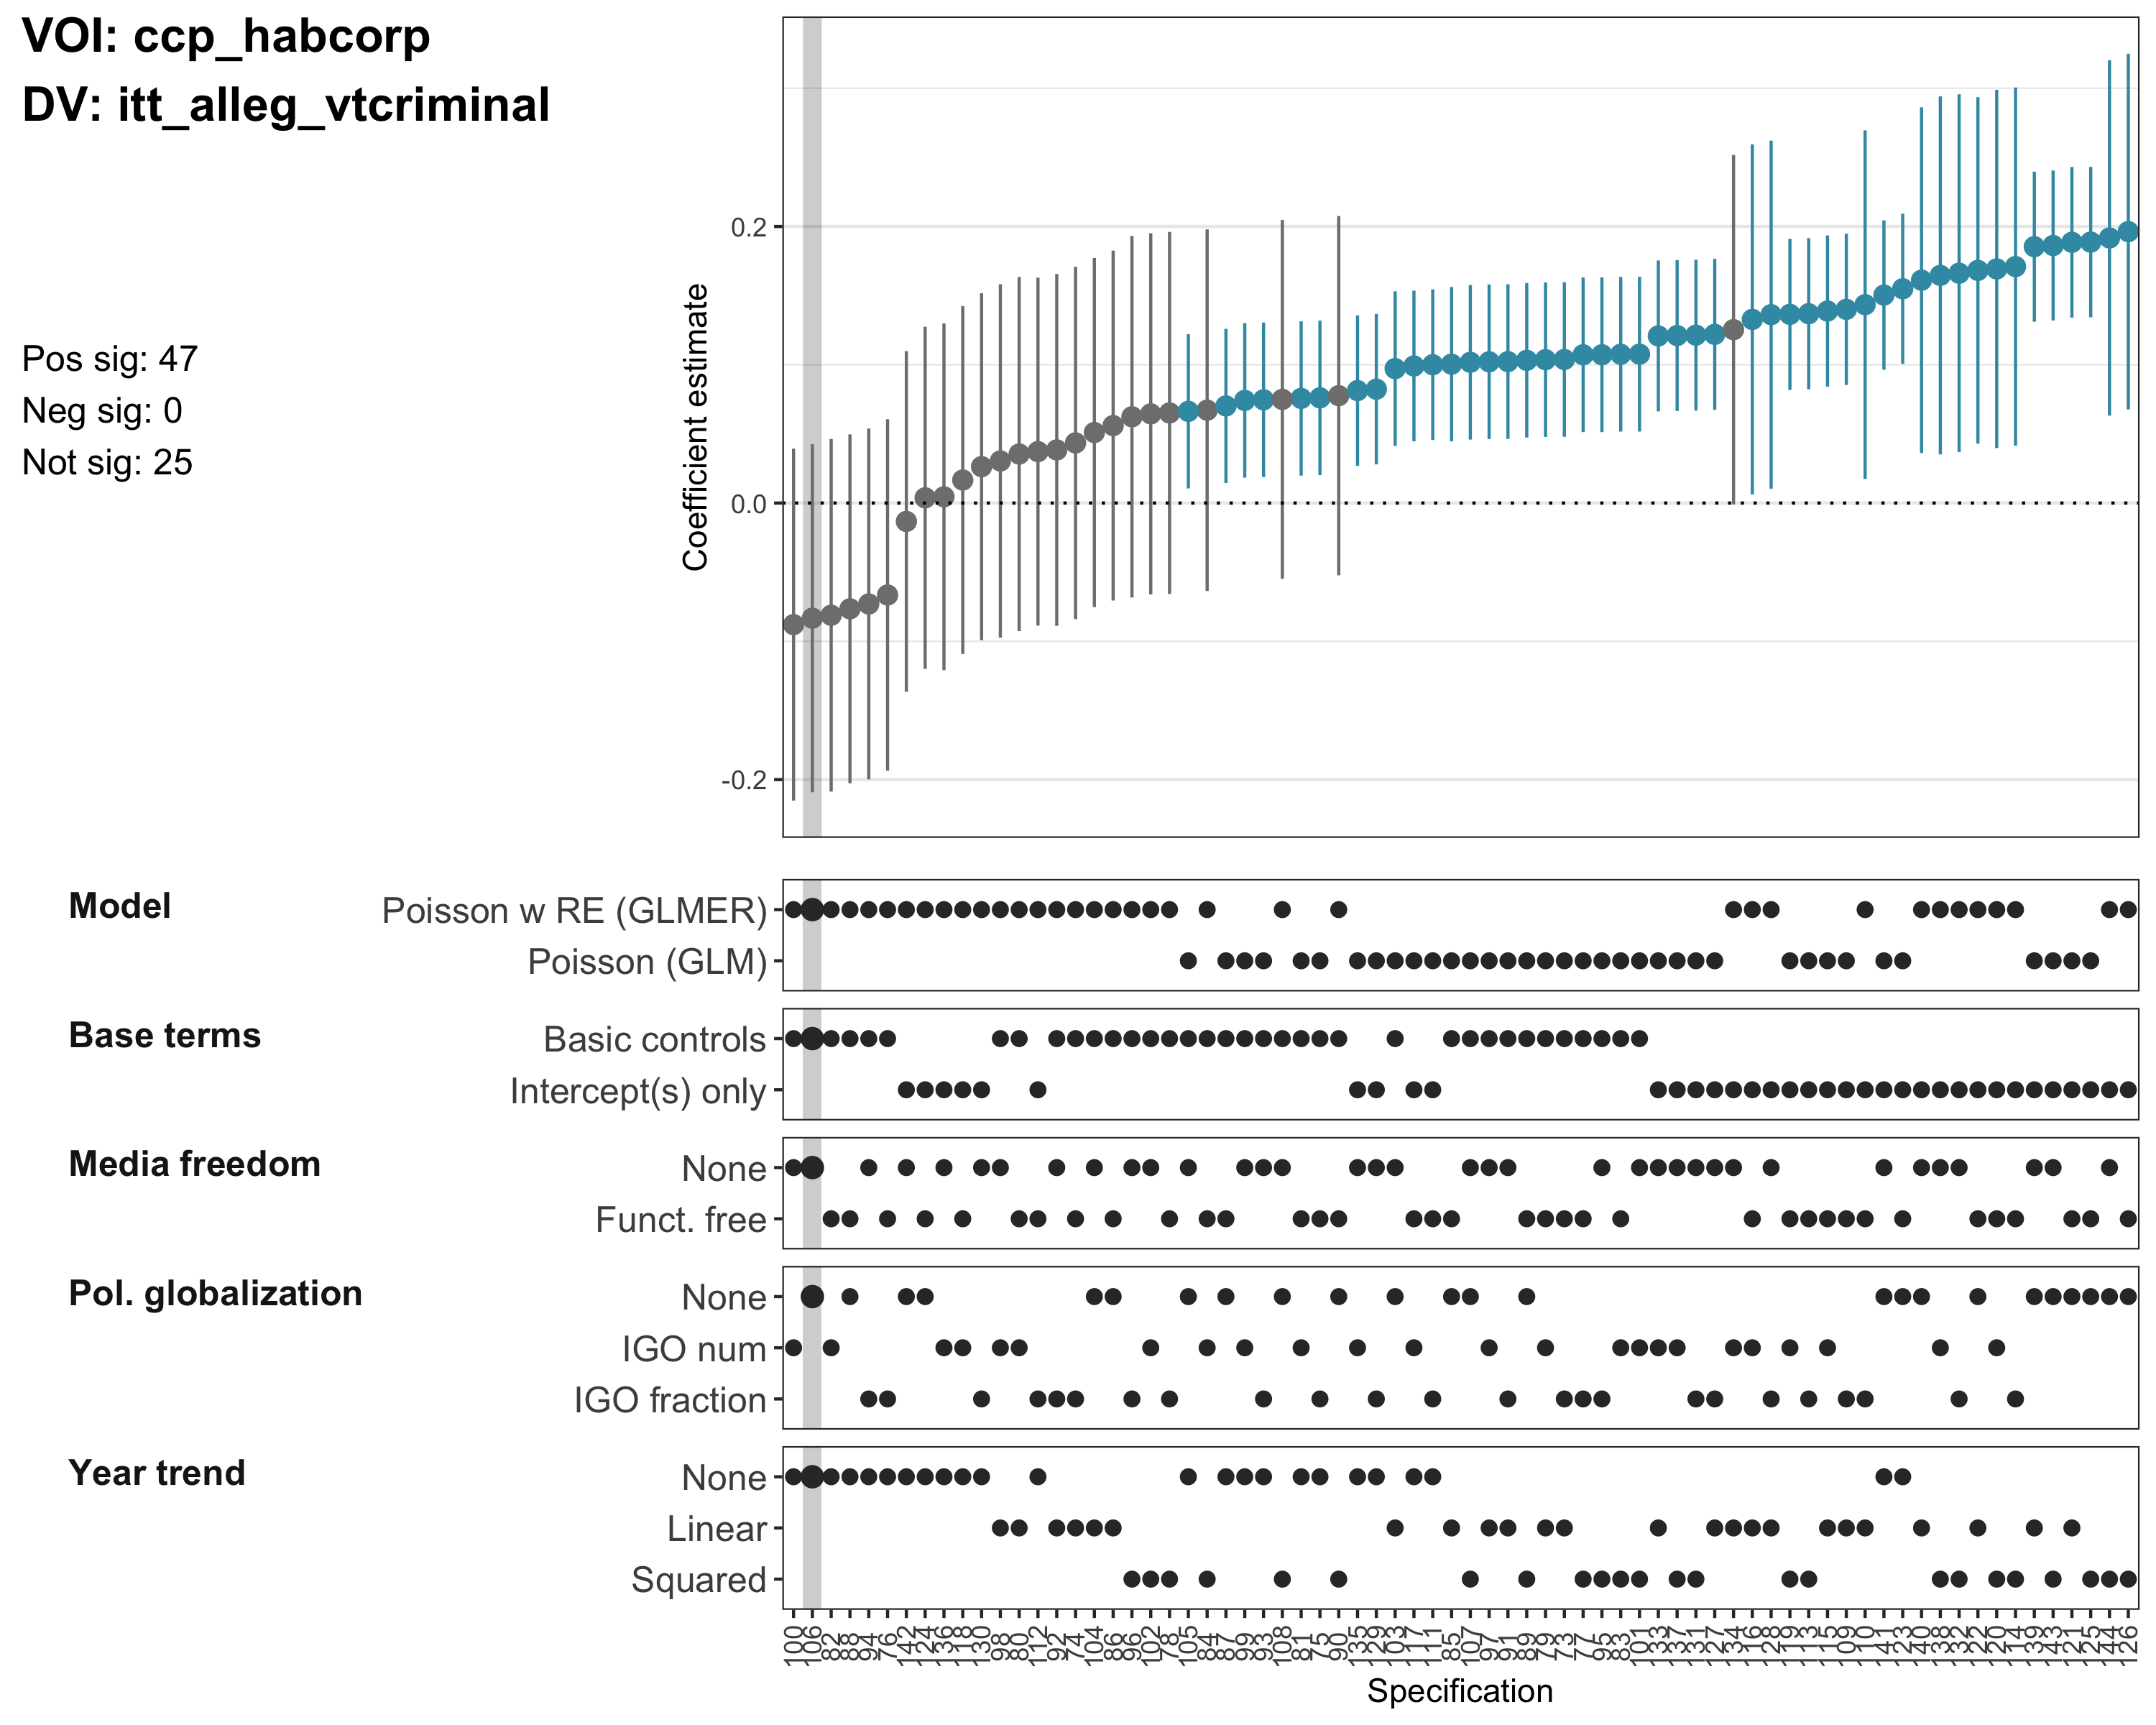
\includegraphics[height=4in]{../output/figures-robustness/specplot-ccp_habcorp-itt_alleg_vtcriminal.png}

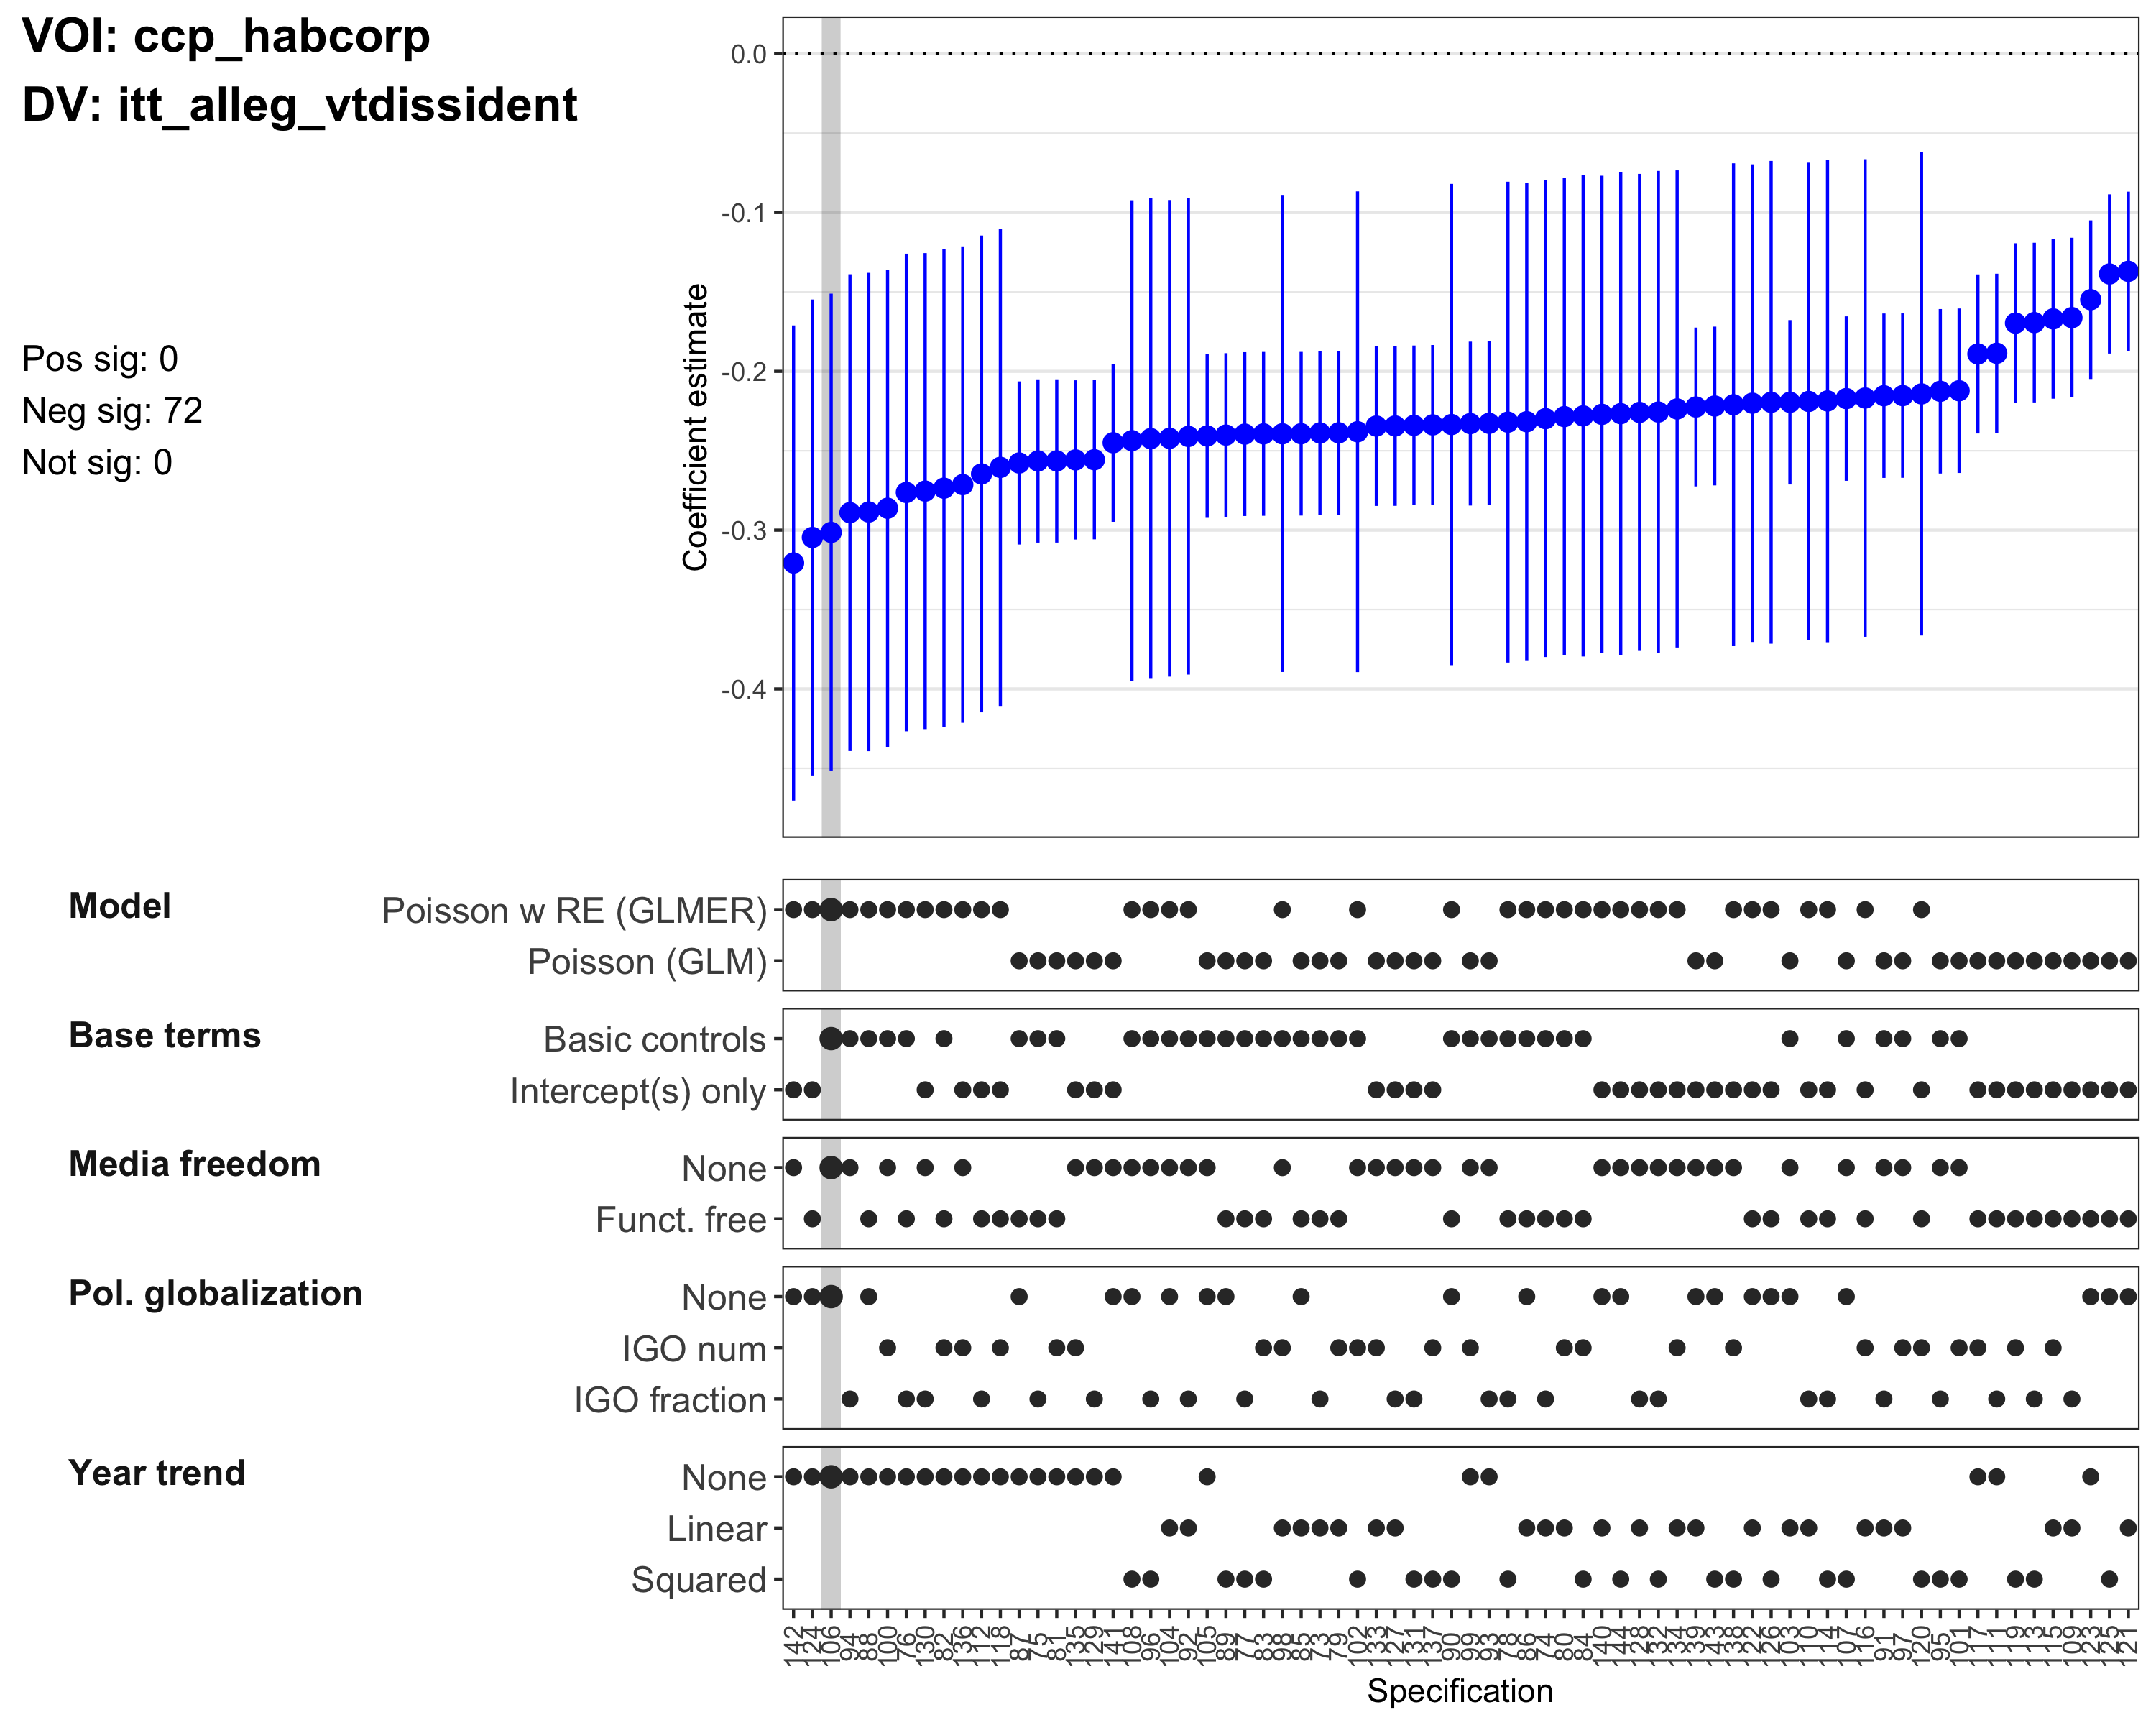
\includegraphics[height=4in]{../output/figures-robustness/specplot-ccp_habcorp-itt_alleg_vtdissident.png}

\hypertarget{references}{%
\section*{References}\label{references}}
\addcontentsline{toc}{section}{References}

\hypertarget{refs}{}
\leavevmode\hypertarget{ref-gelman2013garden}{}%
Gelman, Andrew, and Eric Loken. 2013. ``The garden of forking paths.''
\url{http://www.stat.columbia.edu//textbackslashtextasciitildegelman/research/unpublished/p/_hacking.pdf}.

\leavevmode\hypertarget{ref-simonsohn2015specification}{}%
Simonsohn, Uri, Joseph P Simmons, and Leif D Nelson. 2015.
``Specification Curve: Descriptive and Inferential Statistics on All
Reasonable Specifications.'' \emph{SSRN Electronic Journal}.
\url{https://doi.org/10.2139/ssrn.2694998}.


\end{document}
